The logger is the part that records all the data from the INA260's, and from the clients, to a log directory. This is the main part of our project.
\subsection{Setup} \label{lsetup}
To continue where this project has left of, internet is definitely required. We use a hotspot to do everything that required an internet connection.\newline
The cluster also needs to be setup correctly. Make sure all the power connectors from the black PCB's are connected to the correct Raspberry Pi's. We labelled the Pi's from bottom to top: 0 - 3, with the highest up one being the "g" pi, or Grafana pi. In our setup we conected them to the PCB as follows:
\begin{table}[h]
\centering
\begin{tabular}{|l|l|}
\hline
Address & Pi \\ \hline
0x40 & 0 \\ \hline
0x41 & 1 \\ \hline
0x42 & 2 \\ \hline
0x43 & 3 \\ \hline
0x44 & G \\ \hline
\end{tabular}
\end{table}
\newline
With the addresses being on the following places:
\begin{figure}[h]
	\centering
	\begin{subfigure}[b]{0.4\linewidth}
    		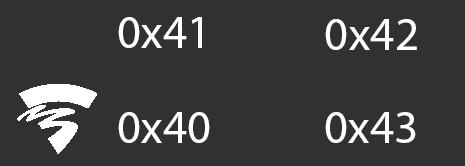
\includegraphics[width=\linewidth]{pcb-ina-0.png}
    		\caption{Bottom PCB}
    	\end{subfigure}
    \begin{subfigure}[b]{0.4\linewidth}
    		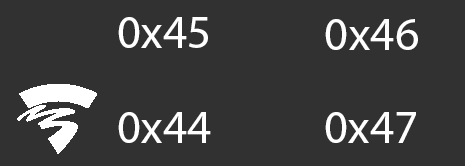
\includegraphics[width=\linewidth]{pcb-ina-1.png}
    		\caption{Top PCB}
    \end{subfigure}
    \caption{PCB INA connector layout, following page 18 of \url{http://www.ti.com/lit/ds/symlink/ina260.pdf}}
    \label{inapcb}
\end{figure}\newline
After that, make sure every Pi has it's own ethernet connection to the switch. If everything is setup correctly, it should work with the provided settings file "pis.xml" in the ina260 folder, the file will be required when starting the logger.\newline
\newline
\textbf{NOTE:}
\begin{itemize}
	\item In the current release of Debian Buster, the Pi picks only one of two interfaces (WiFi or Ethernet). Keep this in mind when trying to connect the Pi's to your hotspot.
\end{itemize}
Now you can make sure the Pi is authorized to access the HvA gitlab servers with an account.
\newline
The last step for setup, also the most essential for running, is to add all the Raspberry Pi's that you want to measure to your \code{/etc/hosts} file. For example, to add \code{raspberrypi-0}, you would write\newline
\code{0.0.0.0 raspberrypi-0.local}\newline
Where \code{0.0.0.0} has to be the actual IP address associated with the hostname. We have not been able to find out why this is necessary, but it seems that the logging programme is not able to do a reverse DNS lookup on it's own.